
\documentclass[aspectratio=1610, 13pt]{beamer}
%\usepackage{ctex}
%\usepackage{CJKutf8}
\usepackage{xcolor}
\usepackage{multicol}
\usepackage{mathtools,array}
\usepackage[T1]{fontenc}
\usepackage{zi4}
\usepackage[font={scriptsize,bf}]{caption}
% \usepackage{subcaption}
\usepackage{graphics}
\usepackage{tikz}
\usepackage{fontawesome5}
\usepackage{mathpartir}

\newcommand{\naturals}{\mathbb{N}}
\newcommand{\reals}{\mathbb{R}}

\newcommand{\Dist}[1]{\mathcal{D}(#1)}
\newcommand{\expectation}{\mathbb{E}}

\newcommand{\states}{S}
\newcommand{\actions}{A}
\newcommand{\observables}{O}
\newcommand{\trans}{T}
\newcommand{\obs}{Z}
\newcommand{\reward}{R}
\newcommand{\discount}{\gamma}

\newcommand{\beliefs}{\mathcal{B}}
\newcommand{\beliefUpdate}{\tau}

\newcommand{\policy}{\pi}

\newcommand{\diff}[1]{\mathop{}\!\mathrm{d}#1}
\renewcommand{\figurename}{Figure}
\renewcommand{\refname}{Reference}

\AtBeginDocument{
  \catcode`_=12
  \begingroup\lccode`~=`_
  \lowercase{\endgroup\let~}\sb
  \mathcode`_="8000
}

% \usetheme{Madrid}
% % \usetheme{default}
% \setbeamertemplate{caption}[numbered]
% \setbeamerfont{title}{size=\large}
\mode<presentation>
{
  \usetheme{Darmstadt}      % or try Darmstadt, Madrid, Warsaw, ...
  \usecolortheme{default} % or try albatross, beaver, crane, ...
  \usefonttheme[onlymath]{serif}  % or try serif, structurebold, ...
  \setbeamertemplate{navigation symbols}{}
  \setbeamertemplate{caption}[numbered]
  \setbeamertemplate{footline}[frame number] 
} 

\usepackage{listings}
\lstdefinestyle{heaplang}{
    language=C,
    basicstyle=\footnotesize\ttfamily,
    keywordstyle=\color{blue},
    commentstyle=\color{red},
    escapeinside={<@}{@>},
    morekeywords={new_chan, fork, recv, send, swap, ref}
}
\lstdefinestyle{clang}{
    language=C,
    basicstyle=\footnotesize\ttfamily,
    keywordstyle=\color{blue},
    commentstyle=\color{red},
    escapeinside={<@}{@>},
}
\lstset{style=heaplang}

\usepackage{natbib}

\newcommand{\buchi}{B\"uchi }

\definecolor{goldenpoppy}{rgb}{0.99, 0.76, 0.0}
\definecolor{goldenyellow}{rgb}{1.0, 0.87, 0.0}
\definecolor{green2}{rgb}{0.1,0.7,0.3} 
\newcommand{\gcheck}{{\color{green2}\faCheckCircle[regular] }}
\newcommand{\rcross}{{\color{red} \faTimesCircle[regular]} }
\newcommand{\rflag}{{\color{red} \faFlag}}
% \usepackage{algorithm,amsmath}
% \usepackage[noend]{algpseudocode}

\newcommand{\zlstinline}{\let\par\endgraf\lstinline}
\newcommand{\comments}[1]{{\color{red}#1}}
\title{Program Analysis - 1}
\date{\today}
\author{Speaker: Xie Li}
\begin{document}
\maketitle

\begin{frame}\frametitle{Overview}
Sources:
\begin{itemize}
\item Principles of Program Analysis, Nielson 1999.
\item Slides of Yingfei Xiong.
\end{itemize}
Contents:
\begin{enumerate}

\item Introduction (\textbf{Part of}).
\item \textbf{Data Flow Analysis}.
\item Constraint Based Analysis.
\item Abstract Interpretation.
\item Type and Effect System.
\end{enumerate}

\end{frame}


\begin{frame}\frametitle{Data Flow Analysis: Preliminaries}
\begin{itemize}
\item \textbf{Preliminaries on Partial Ordered Sets}.
\item Reaching Definition Analysis.
\item Live Variables Analysis.
\item Theoretical Properties.


\end{itemize}
\end{frame}





\begin{frame}\frametitle{Preliminaries}
\begin{definition}[Partial Order Set]
\begin{center}

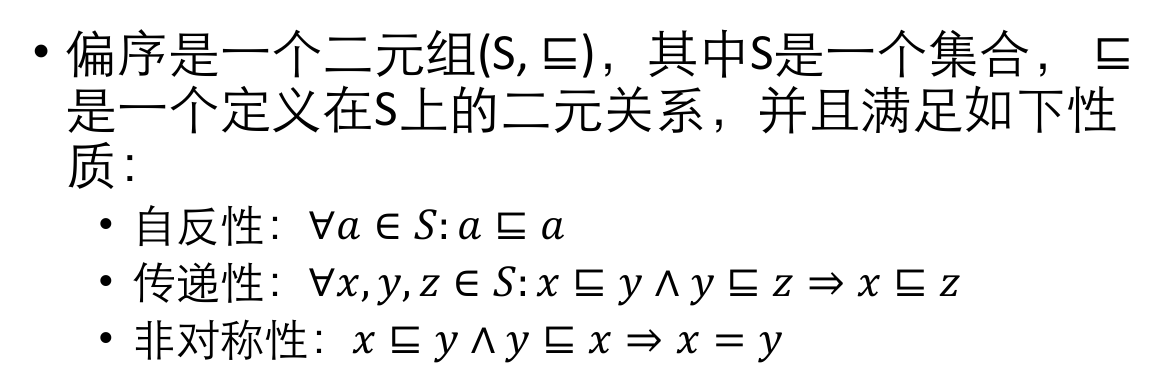
\includegraphics[scale=0.23]{pos.png}
\end{center}

\end{definition}
\begin{itemize}
\item \emph{Upper bound}: A subset $Y$ of $S$ has $l\in S$ as upper bound if $\forall l'\in Y. l' \sqsubseteq l$.
\item \emph{Greatest upper bound}: $l\in S$ is the greatest upper bound of $Y$ iff forall upper bounds $l_0\in S$, $l \sqsubseteq l_0$.
\item 
Similar definition for lower bound and least lower bound.

\end{itemize}

We use $\sqcap Y$ and $\sqcup Y$ to represent the greatest lower bound (meet) and least lower bound (join) of $Y$. 

$l_1 \sqcap l_2, l_1 \sqcup l_2$.

\end{frame}


\begin{frame}\frametitle{Complete Lattice}
\begin{definition}[Complete Lattice]
A \emph{complete lattice} $L = (L, \sqsubseteq) = (L, \sqsubseteq, \sqcup, \sqcap, \top, \perp)$.

\end{definition}
\begin{example}
A complete lattice defined on the superset of $\{1,2,3\}$ where the partial order is $\subseteq$.
\begin{center}
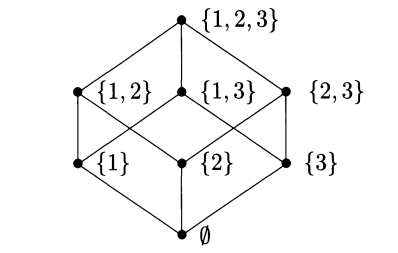
\includegraphics[scale=0.4]{complete_lattice_example.png}
\end{center}
\end{example}
\end{frame}

\begin{frame}\frametitle{Monotone Function}
\begin{definition}[Monotone Function]
A \emph{monotone function} is a function $f: L_1 \rightarrow L_2$ between partially ordered sets $(L_1, \sqsubseteq_1)$ and $(L_2, \sqsubseteq_2)$ s.t.
\[\forall l, l' \in L_1. (l \sqsubseteq_1 l' \implies f(l) \sqsubseteq_2 f(l'))\]

\end{definition}

\begin{example}
The monotone (increasing) function from $(\mathbb{R}, \le)$ to $(\mathbb{R}, \le)$.

\end{example}
\end{frame}

\begin{frame}\frametitle{Fixed Points}
Given a complete lattice $(L, \sqsubseteq, \sqcup, \sqcap, \top, \perp)$,
\begin{multicols}{2}
\begin{center}
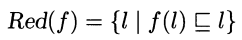
\includegraphics[scale=0.4]{red.png}

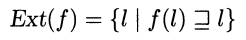
\includegraphics[scale=0.4]{ext.png}

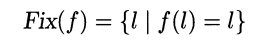
\includegraphics[scale=0.4]{fix.png}
\end{center}
Least fix-point and greatest fix-point:
\begin{center}
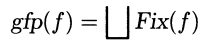
\includegraphics[scale=0.4]{gfp.png}

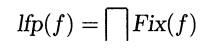
\includegraphics[scale=0.4]{lfp.png}
\end{center}


\begin{center}
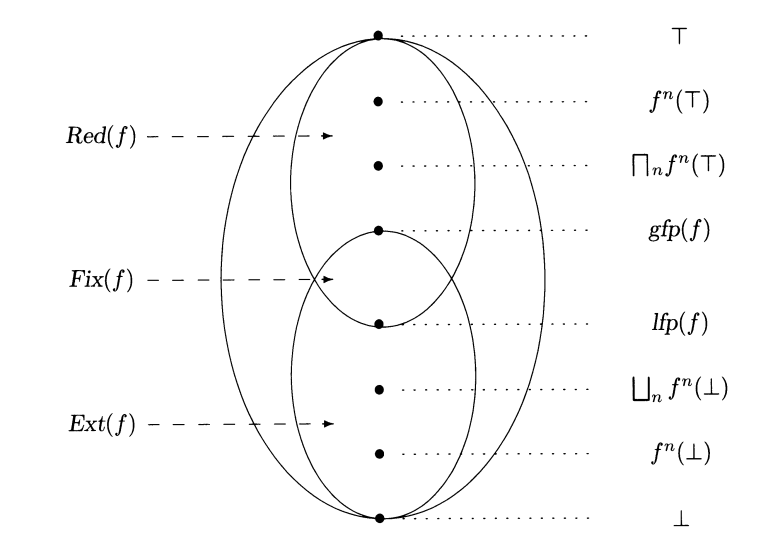
\includegraphics[scale=0.27]{fixpoint_pic.png}
\end{center}
\end{multicols}
\end{frame}

\begin{frame}\frametitle{Tarski Fixed Point Theorem}

\begin{center}
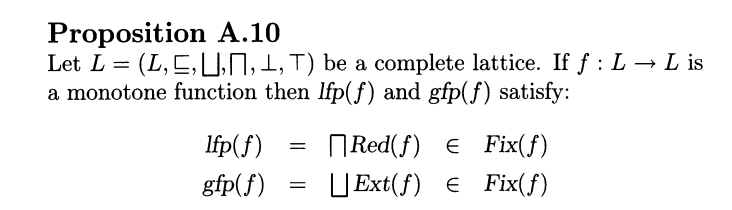
\includegraphics[scale=0.4]{tarski.png}

\end{center}
Proof.

\begin{center}

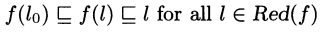
\includegraphics[scale=0.4]{proof_tarski.png}
\end{center}

\end{frame}


\begin{frame}\frametitle{Data Flow Analysis}
\begin{itemize}

\item Preliminaries on Partial Ordered Sets.
\item \textbf{Reaching Definition Analysis}.
\item Live Variables Analysis.
\item Theoretical Properties.


\end{itemize}
\end{frame}

\begin{frame}\frametitle{Basic Notations}
\begin{center}
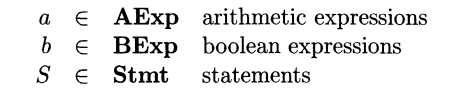
\includegraphics[scale=0.4]{not1.png}
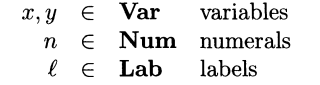
\includegraphics[scale=0.4]{not2.png}

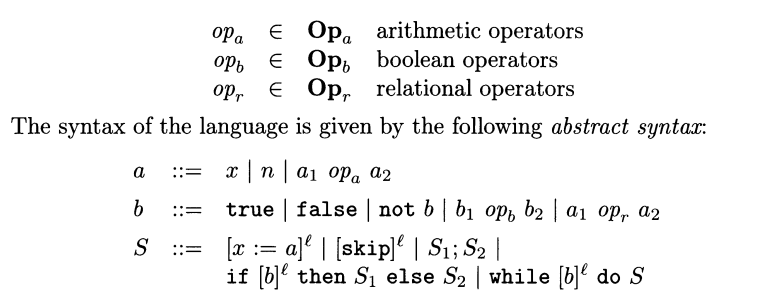
\includegraphics[scale=0.4]{not3.png}
\end{center}
\end{frame}

\begin{frame}\frametitle{Example of Program}
\begin{center}
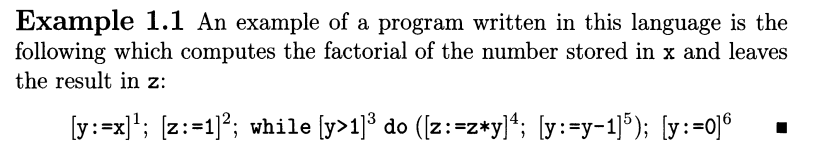
\includegraphics[scale=0.4]{prog_example1.png}

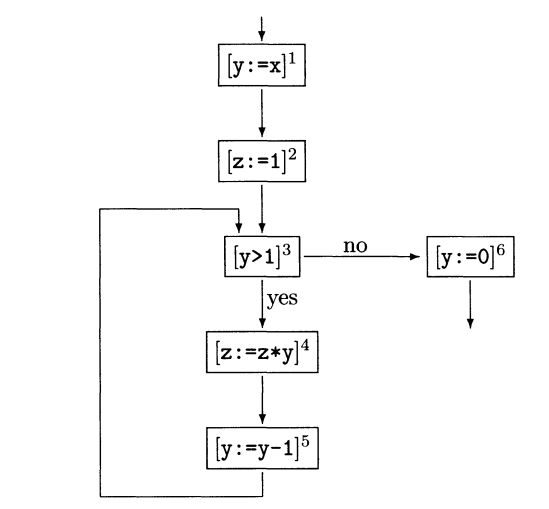
\includegraphics[scale=0.3]{proc_flowgraph.png}
\end{center}
\end{frame}

\begin{frame}\frametitle{Other Notations}

\[init,final,blocks,labels,flow,flow^{R}\]

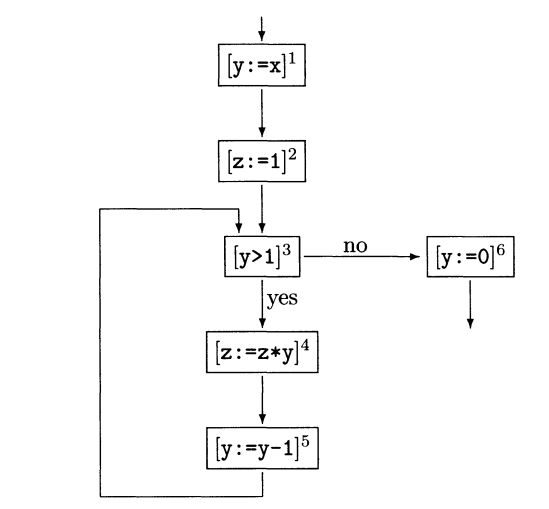
\includegraphics[scale=0.3]{proc_flowgraph.png}
\end{frame}

\begin{frame}\frametitle{Reaching Definition Analysis}
\begin{multicols}{2}
\textbf{Reaching definition}: An assignment of the form $[x := a]^l$ \textit{may reach} a certain program point if there is an execution of the program where $x$ was last assigned at value at $l$ when the program point is reached.

\textbf{Program points}: exits and entries of elementary blocks.


\textbf{Problem}: For each program points, find a set of pairs like $(x,l)$ to represent the assignment that may reach the program points.


\textbf{Notations}: $(x, ?), (x, l)$
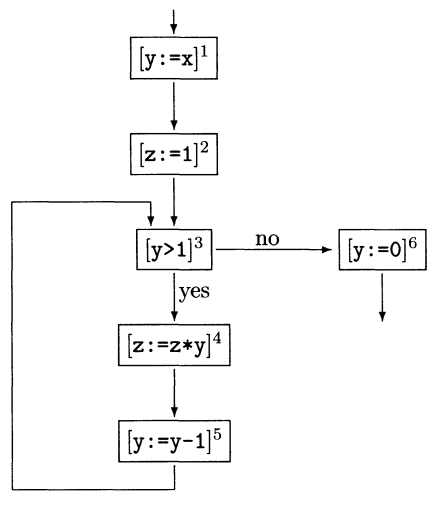
\includegraphics[scale=0.35]{small_demo.png}
\end{multicols}
\end{frame}

\begin{frame}\frametitle{Data Flow Analysis: Equational Approach}
\begin{center}

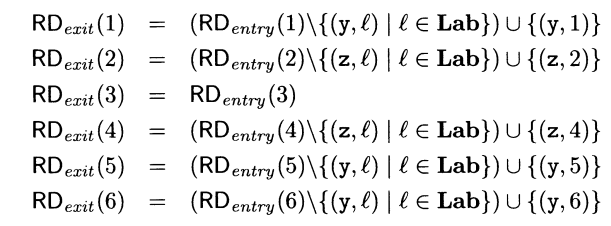
\includegraphics[scale=0.4]{rd_eq1.png}
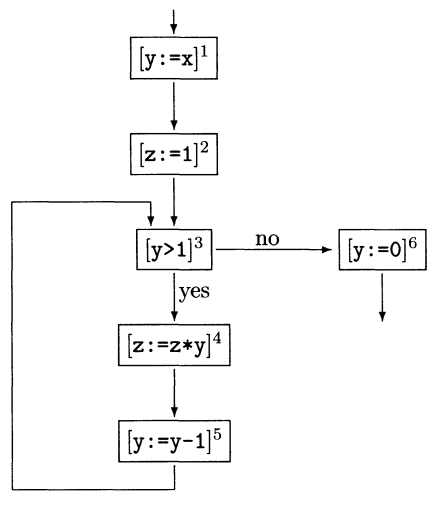
\includegraphics[scale=0.3]{small_demo.png}
\end{center}


\end{frame}

\begin{frame}\frametitle{Data Flow Analysis: Equational Approach}
\begin{multicols}{2}
\begin{center}


\includegraphics[scale=0.4]{rd_eq2.png}

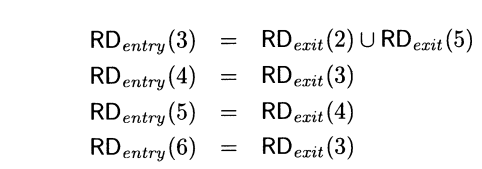
\includegraphics[scale=0.4]{rd_eq3.png}

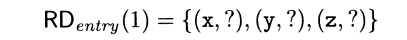
\includegraphics[scale=0.4]{rd_eq4.png}
\end{center}
\begin{center}

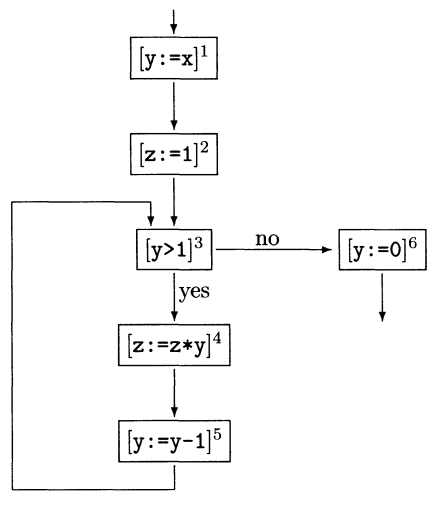
\includegraphics[scale=0.3]{small_demo.png}
\end{center}
\end{multicols}
\end{frame}

\begin{frame}\frametitle{How these equations generated?}
Forward analysis.
\begin{center}
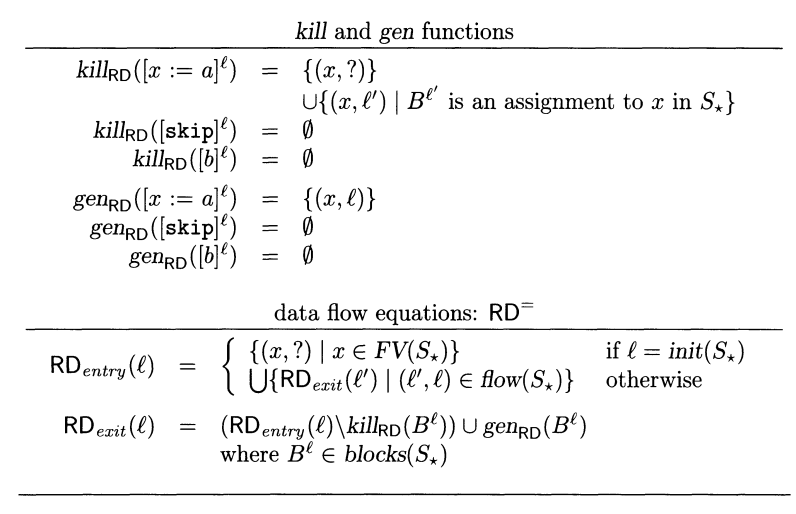
\includegraphics[scale=0.4]{rd_analysis.png}
\end{center}
\end{frame}

\begin{frame}\frametitle{Solve the equation system.}
For the above program we obtain twelve sets at the program points:
\[\vec{\texttt{RD}} = (\texttt{RD}_{entry}(1), \texttt{RD}_{exit}(1), \ldots, \texttt{RD}_{entry}(6), \texttt{RD}_{exit}(6))\]

We can regard one step execution of the program as a function $F$ on $\vec{\texttt{RD}}$. i.e. 

\begin{center}
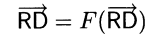
\includegraphics[scale=0.4]{eq_system.png}

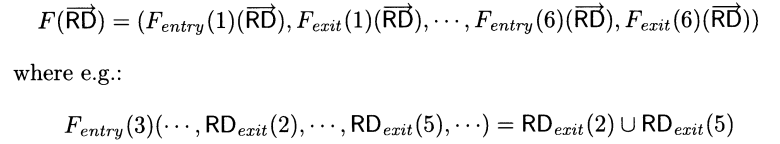
\includegraphics[scale=0.4]{eq_system_example.png}
\end{center}

\end{frame}

\begin{frame}\frametitle{Solve the equation system.}
Definition of the function $F$:
\begin{center}
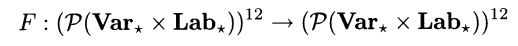
\includegraphics[scale=0.4]{rd_func.png}
\end{center}
Partial order for the complete lattice:
\begin{center}
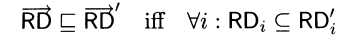
\includegraphics[scale=0.4]{rd_cl.png}
\end{center}
$F$ is a monotone function:
\begin{center}
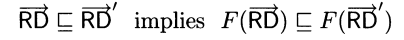
\includegraphics[scale=0.4]{rd_monotone.png}
\end{center}
Fix-point of $F$ is the least solution to the equation system.
\begin{center}
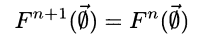
\includegraphics[scale=0.4]{rd_fixpoint.png}

\end{center}

\end{frame}



\begin{frame}\frametitle{Data Flow Analysis: Live Variable Analysis}
\begin{itemize}
\item Reaching Definition Analysis.
\item Preliminaries on Partial Ordered Sets.
\item \textbf{Live Variables Analysis}.
\item Theoretical Properties.


\end{itemize}
\end{frame}



\begin{frame}[fragile]\frametitle{Live Variable Analysis}
\textbf{Live variable:}  varDef $\longrightarrow$ varUsed

Along the path, there is no redefinition to the variable.

Then we call it live at the exit of the program.

\textbf{Problem:} for each program point, which variable \textit{may} be live at the exit from the point.
\begin{example}
\begin{lstlisting}
int main(){
    int x = 10;
    int y = 11;
    int z = x + 1;
    return z;
}

\end{lstlisting}

\end{example}

Live variable analysis is useful in dead code elimination.
\end{frame}


\begin{frame}\frametitle{Live Variable Analysis}
Backward analysis. Smallest solution.
\begin{center}
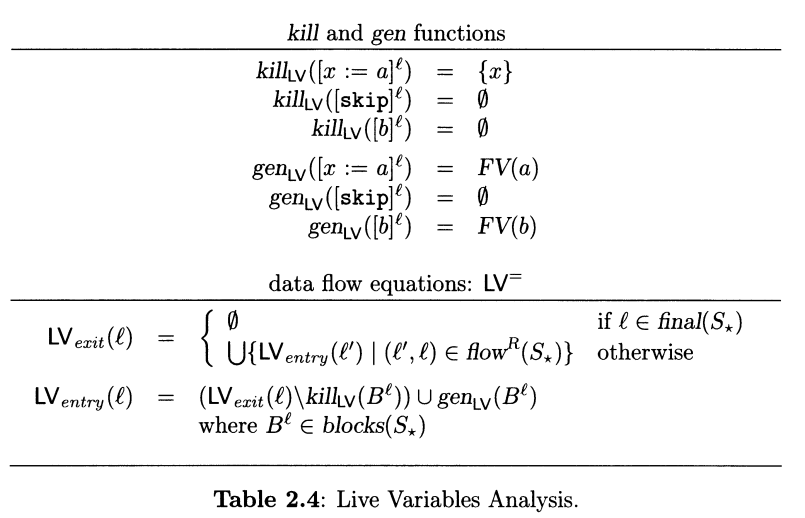
\includegraphics[scale=0.4]{lv.png}
\end{center}
\end{frame}

\begin{frame}\frametitle{The Difference between May and Must}

\begin{center}
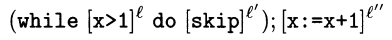
\includegraphics[scale=0.4]{lv_example.png}

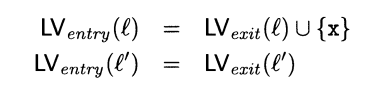
\includegraphics[scale=0.4]{lv_ex_eq.png}

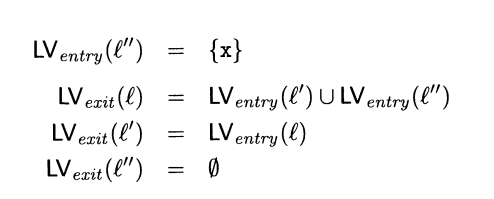
\includegraphics[scale=0.4]{lv_ex_eq2.png}
\end{center}
After some calculations:
\begin{center}
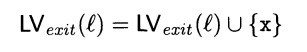
\includegraphics[scale=0.4]{simplified.png}
\end{center}
\end{frame}

\begin{frame}\frametitle{The Difference between May and Must}



\end{frame}


\begin{frame}\frametitle{Monotone Framework}
\begin{center}
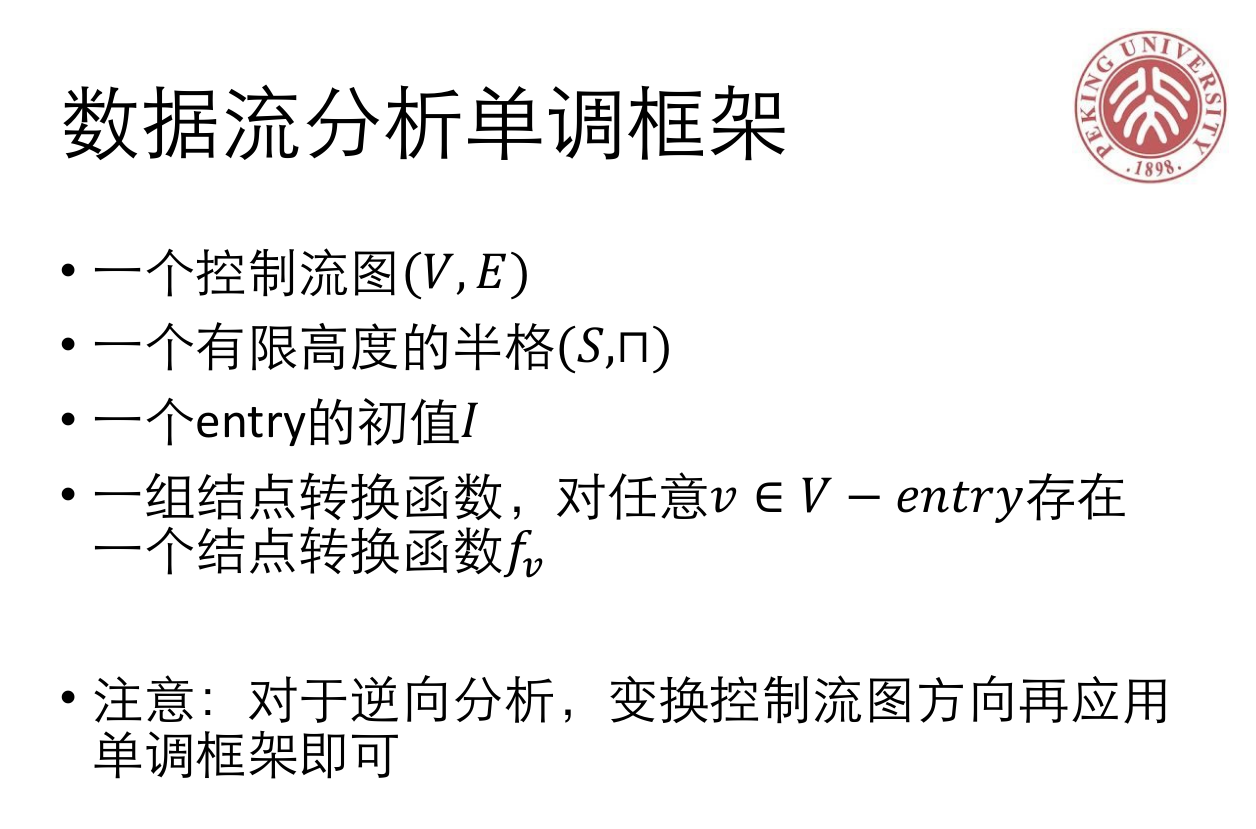
\includegraphics[scale=0.25]{framework.png}
\end{center}
\end{frame}

\begin{frame}\frametitle{Algorithm of Dataflow Analysis}
\begin{center}
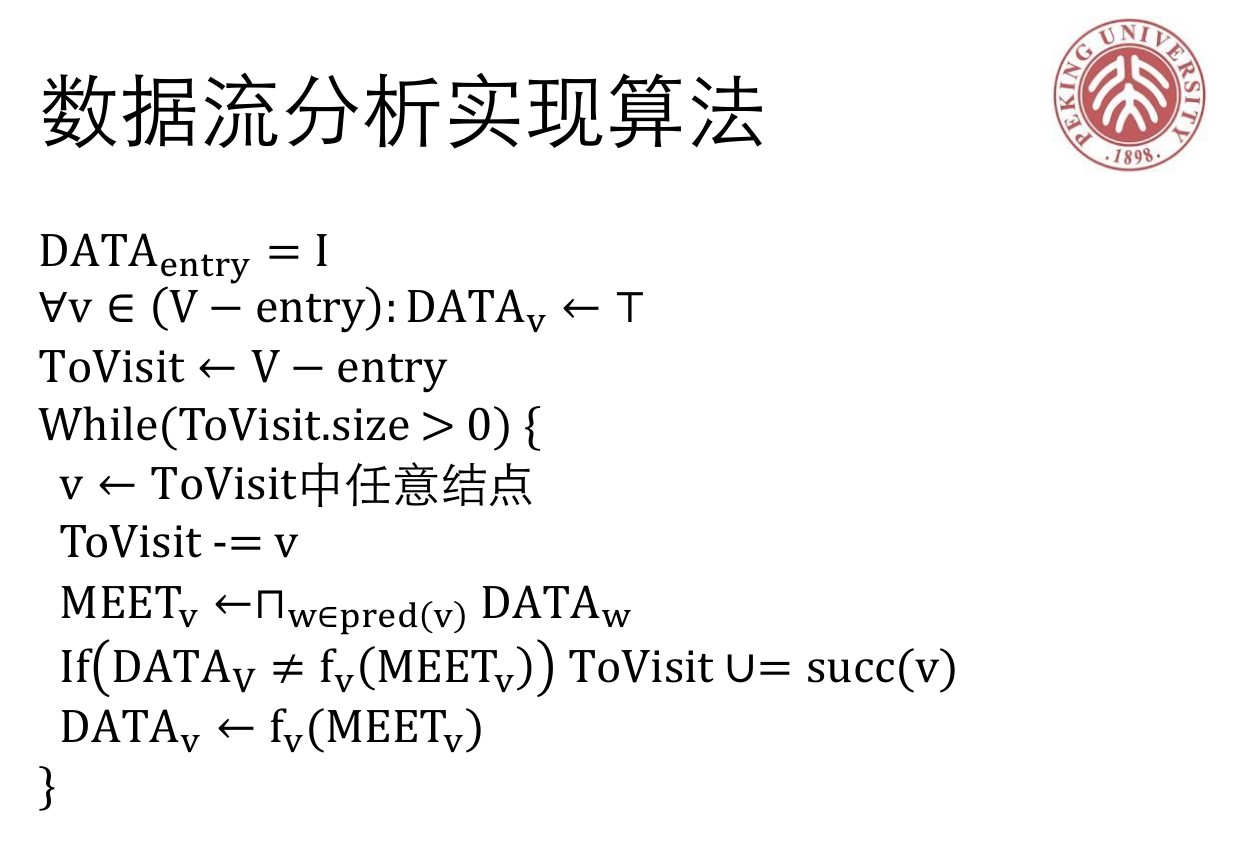
\includegraphics[scale=0.25]{algorithm.png}

\end{center}
\end{frame}

\begin{frame}\frametitle{Data Flow Analysis: Live Variable Analysis}
\begin{itemize}
\item Reaching Definition Analysis.
\item Preliminaries on Partial Ordered Sets.
\item Live Variables Analysis.
\item\textbf{Theoretical Properties}.


\end{itemize}
\end{frame}
\begin{frame}\frametitle{Theoretical Properties}

 
 
\end{frame}



\end{document}